    \tikzstyle{linha} = [line width=1.05mm, rounded corners=1mm, yellow!60]
    \tikzstyle{caixa} = [rectangle, draw=yellow!60, fill=yellow!60, text width=2cm, text centered, minimum height=0.75cm, font=\footnotesize, rounded corners] 
    \tikzstyle{caixalarga} = [rectangle, draw=yellow!35, fill=yellow!60, text width=6cm, text centered, minimum height=0.75cm, font=\footnotesize, rounded corners ]
    \begin{tikzpicture}[>={Triangle[angle=60:3mm]}]
    % PICTURE
	\node at (0,0) (LabPick) {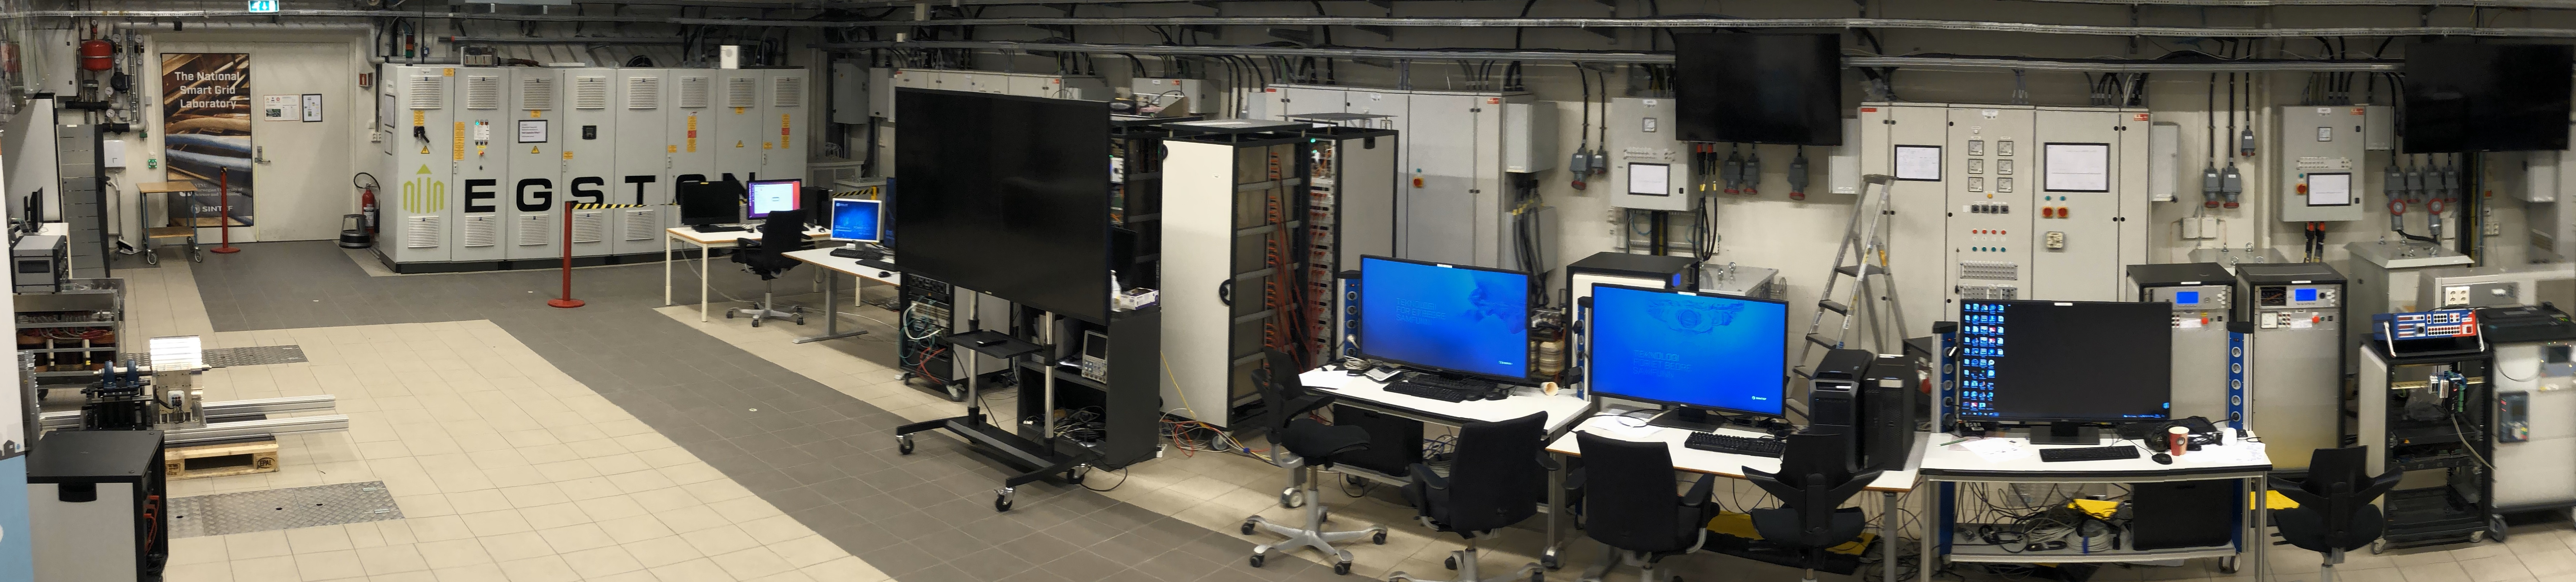
\includegraphics[width=18cm]{figures/SmartGridLab.jpg}};
	% TEXTBOXES
	\node at (-7.5,-1.5) (RTS) [caixa] {Real-Time Simulator};
	\node at (-4.5,-1.5) (GridEmu) [caixa] {Grid Emulator\\AC \& DC };
	\node at (-1.5,-1.5) (ESSTR) [caixa] {Transformer\\ESSTR};
	\node at (3.5,-1.5) (ESSGC) [caixalarga] {Power Electronic Converter\\ESSGC, ESSC$_\textrm{ac}$,
	ESSR$_\textrm{ac}$, ESSL$_\textrm{ac}$, and ESSC$_\textrm{dc}$};
	% ARROWS
	\draw [->, linha] (RTS) -- ++(0,2) -- ++(-0.75,0);
	\draw [->, linha] (GridEmu) -- ++(0,1) -- ++(-1.25,0) -- ++(0,0.65);
	\draw [->, linha] (ESSGC) -- ++(0,2.15) -- ++(2.7,0) -- ++(0,-0.5);
	\draw [->, linha] (ESSTR) -- ++(0,3) -- ++(9.25,0) -- ++(0,-1.2);
	\end{tikzpicture}
